\documentclass[UKenglish]{beamer}


\usetheme[NoLogo]{MathDept}


\usepackage[utf8]{inputenx} % For æ, ø, å
\usepackage[spanish]{babel}          % Automatic translations
\usepackage{csquotes}       % Quotation marks
\usepackage{microtype}      % Improved typography
\usepackage{amssymb}        % Mathematical symbols
\usepackage{mathtools}      % Mathematical symbols
\usepackage{graphicx}
\usepackage[absolute, overlay]{textpos} % Arbitrary placement
\setlength{\TPHorizModule}{\paperwidth} % Textpos units
\setlength{\TPVertModule}{\paperheight} % Textpos units
\usepackage{tikz}
\usetikzlibrary{overlay-beamer-styles}  % Overlay effects for TikZ


\author{Rudik Roberto Rompich}
\title{\textit{Kepler – 442b}\\ – Exotierras en la zona habitable}
\subtitle{\texttt{Introducción a la astronomía}}


\begin{document}

\usebackgroundtemplate{%
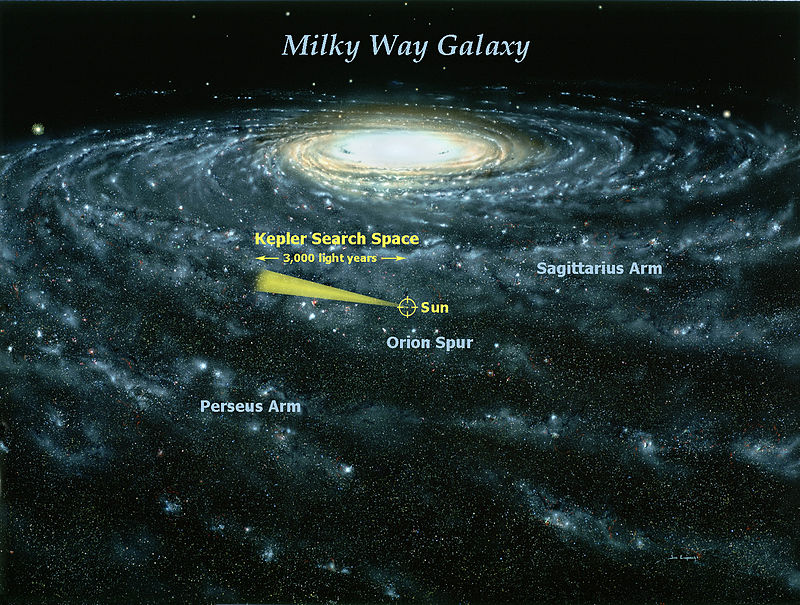
\includegraphics[width=\paperwidth,height=\paperheight]{Imagenes/1}}
  
\section{\textcolor{white}{}}
\SectionPage 
\usebackgroundtemplate{ } 

\section{Índice}


% Use
%
%  \begin{frame}[allowframebreaks]{Title}
%
% if the TOC does not fit one frame.
\begin{frame}[allowframebreaks]{Índice}
    \tableofcontents[currentsection]
\end{frame}


\section{Sistema Planetario}

\begin{frame}
\frametitle{Sistema Planetario}

\begin{columns}

\column{0.4\textwidth}
El planeta \textbf{Kepler 442b} se ubica en el sistema planetario Kepler 442.\\
Datos interesantes: 

\begin{itemize}
\item Un sistema nombrado en honor a la sonda Kepler.
\item 1,206 $\pm$  9 ly
\item 370 $\pm$ 3 pc
\item Lyra
\item 19h 01m 27.98s, +39$^{\circ}$ 16' 48.30''
\end{itemize}

\column{0.4\textwidth}

  \begin{figure}[t!]
    \centering
    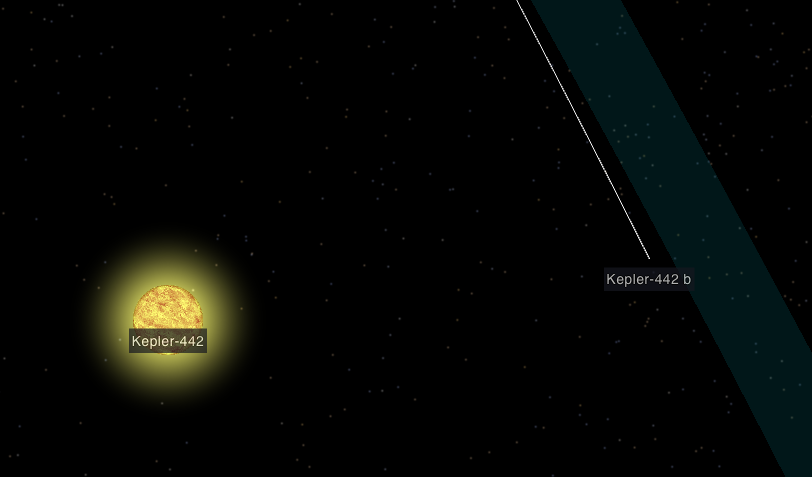
\includegraphics[scale=0.2]{Imagenes/5}
    \caption{Kepler 442 — NASA Exploration}
    \label{fig:punt4os}
    \end{figure}
\end{columns}
\end{frame}


\begin{frame}
\frametitle{Sistema Planetario}{\textbf{19h 01m 27.98s, +39$^{\circ}$ 16' 48.30''}}
\begin{figure}[h!]
    \centering
    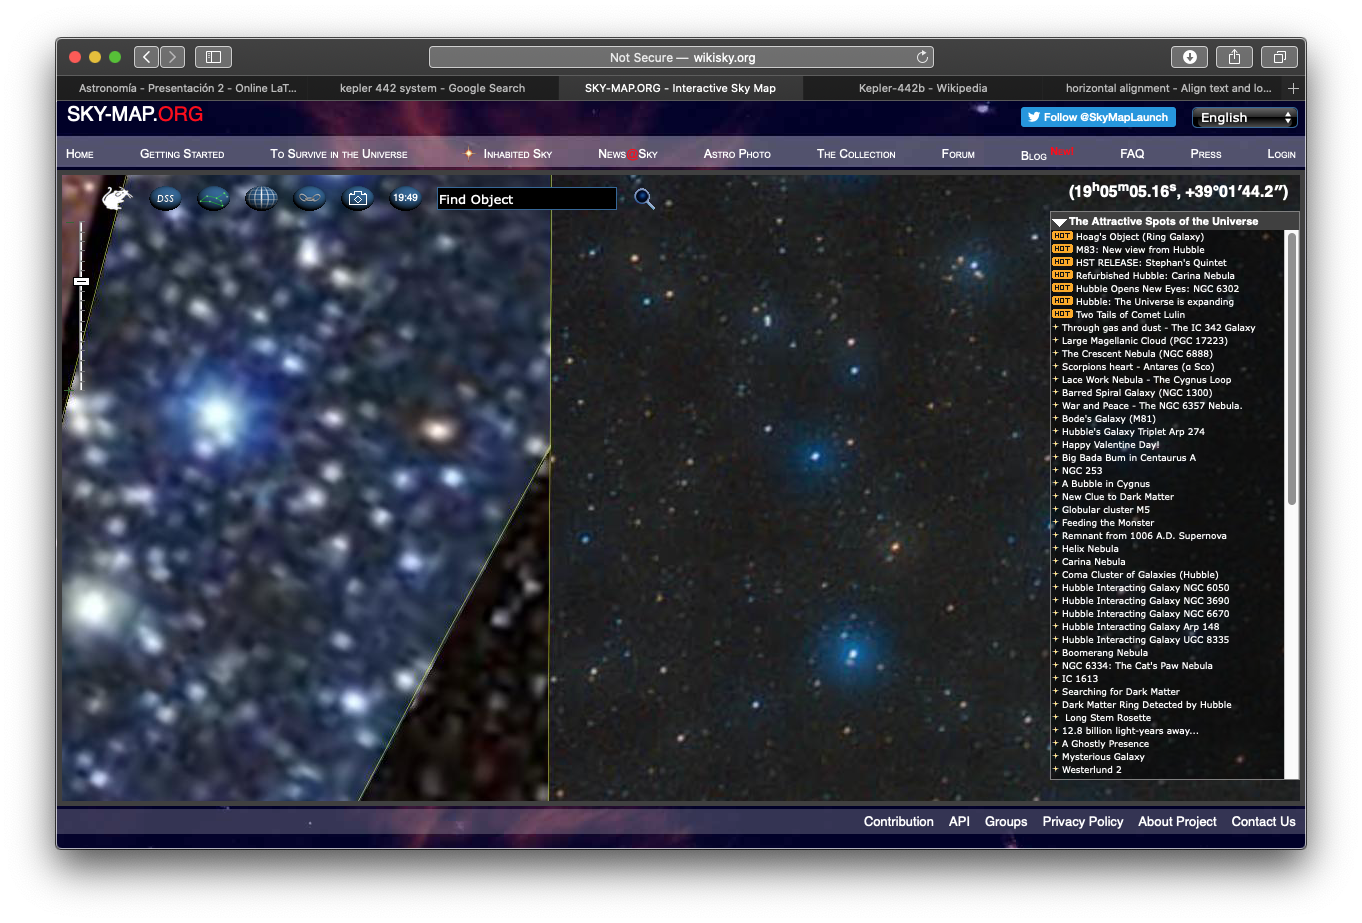
\includegraphics[scale=0.2]{Imagenes/3}
    \caption{19h 01m 27.98s, +39$^{\circ}$ 16' 48.30''}
    \label{fig:pun2tos6}
    \end{figure}
\end{frame}

\begin{frame}
\frametitle{Sistema Planetario}
\begin{figure}[h!]
    \centering
    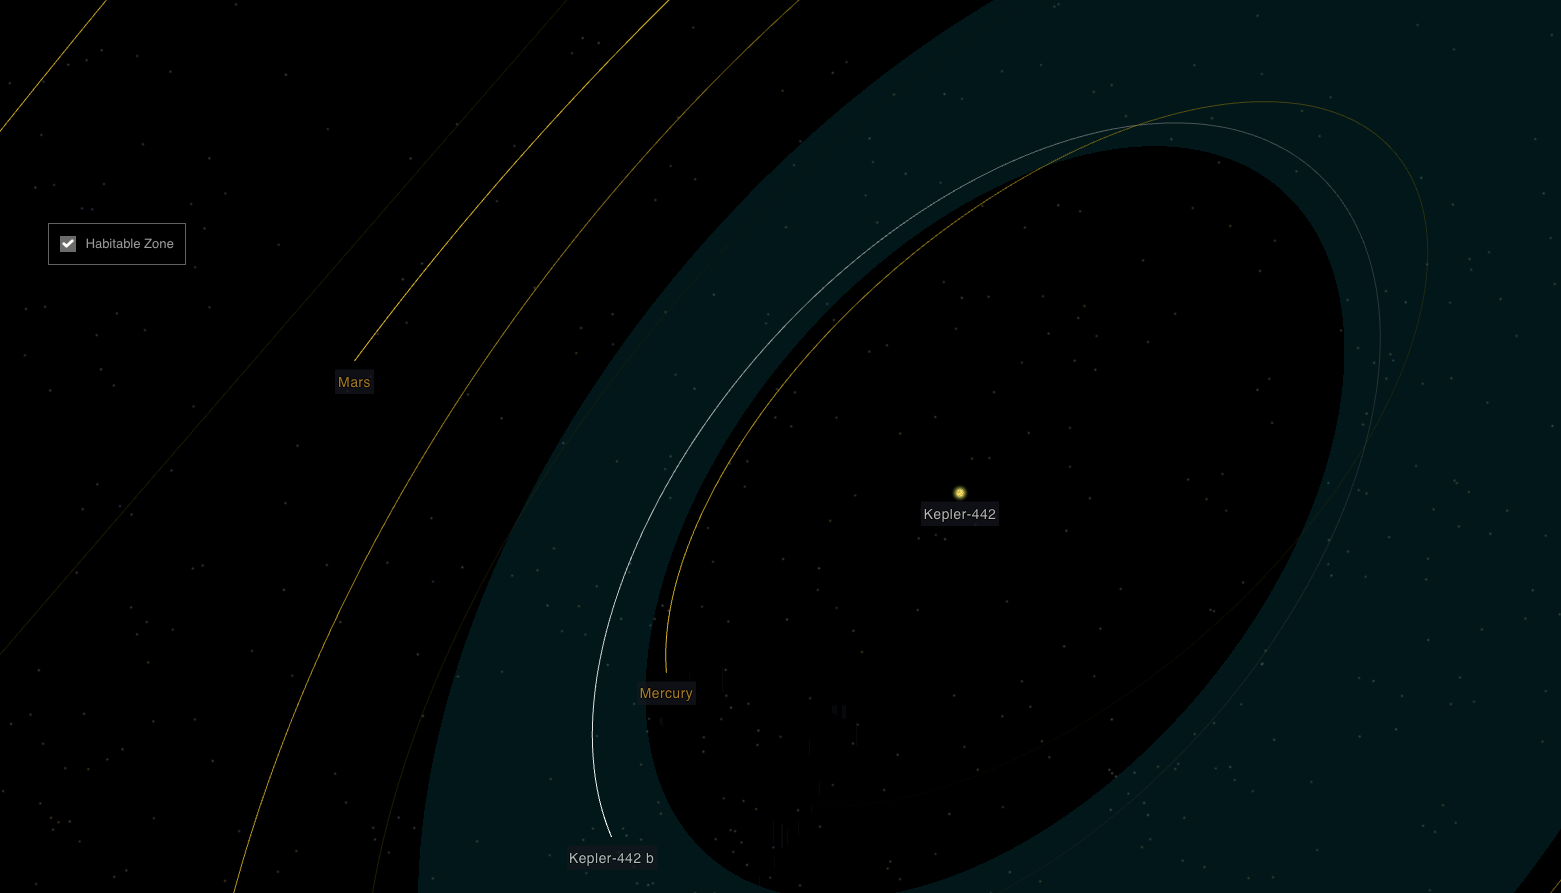
\includegraphics[scale=0.2]{Imagenes/6}
    \caption{Comparación a la órbita de mercurio}
    \label{fig:pun2tos}
    \end{figure}
\end{frame}


\section{Características del planeta}

\begin{frame}
\frametitle{Características del planeta}{\textbf{Descripción}}

\begin{columns}

\column{0.4\textwidth}
Kepler 442b. (2015) Descubierto por medio del método de tránsito. \\
Puntos interesantes:
\begin{itemize}
\item NASA/20 científicos
\item The Astrophysical Journal
\item Enero - Febrero 2020 
\item 12 planetas
\item BLENDER
\end{itemize}

\column{0.4\textwidth}

  \begin{figure}[h!]
    \centering
    \includegraphics[scale=0.12]{Imagenes/Plat}
    \caption{Kepler 442b — NASA Exploration}
    \label{fig:punto2s}
    \end{figure}
\end{columns}
\end{frame}

\begin{frame}
\frametitle{Sistema Planetario}
\begin{figure}[h!]
    \centering
    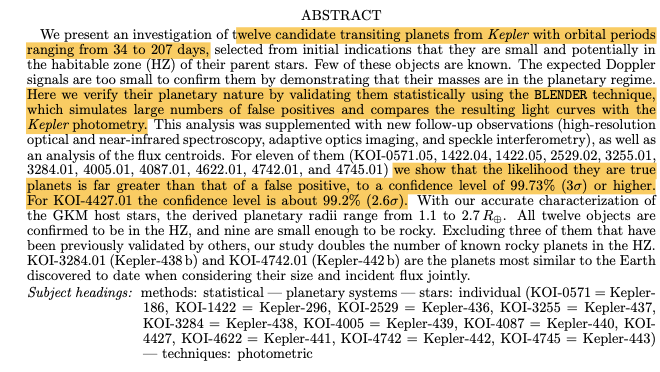
\includegraphics[scale=0.45]{Imagenes/8}
    \caption{BLENDER}
    \label{fig:pun2tosja}
    \end{figure}
\end{frame}

\begin{frame}
\frametitle{Características del planeta}{\textbf{Descripción}}

\begin{columns}

\column{0.4\textwidth}
\begin{figure}[h!]
    \centering
    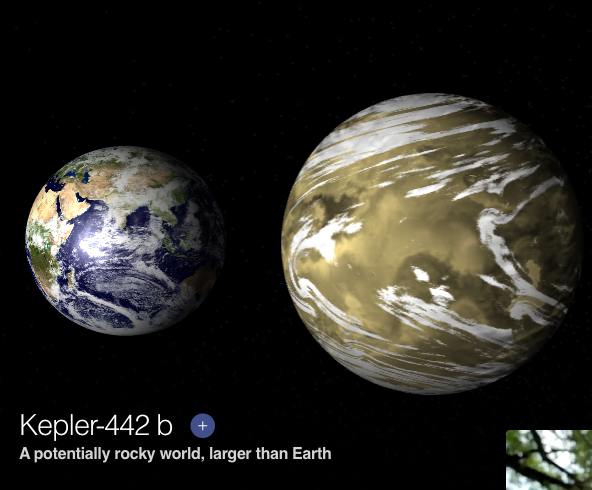
\includegraphics[scale=0.2]{Imagenes/7}
    \caption{Comparación a la tierra}
    \label{fig:puntos}
    \end{figure}

\column{0.4\textwidth}
    Datos puntuales: 
    \begin{itemize}
        \item Súper tierra
        \item Masa: 2.36T 
        \item Radio: 1.34T
        \item PO: 112.3 días
        \item Excentricidad: 0.04
        \item 0.409 AU 
    \end{itemize}
    \end{columns}

\end{frame}

\begin{frame}
\frametitle{Descubrimiento}
\begin{figure}[h!]
    \centering
    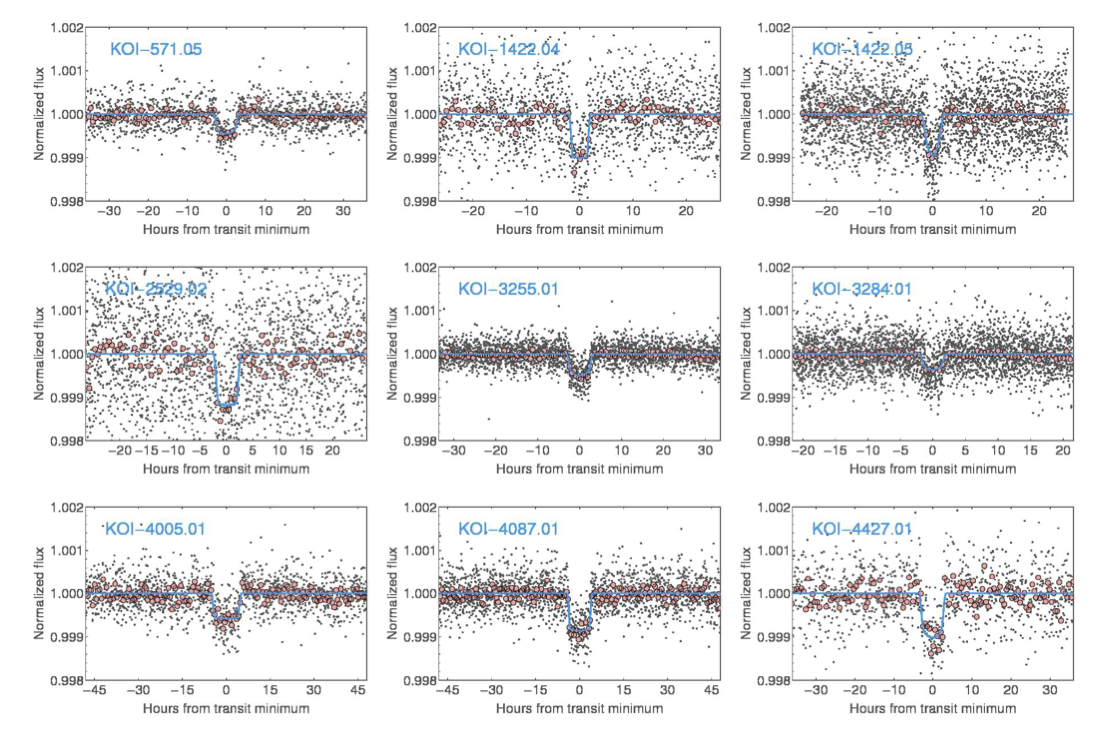
\includegraphics[scale=0.24]{Imagenes/4}
    \caption{Sistema}
    \label{fig:transicion}
    \end{figure}
\end{frame}

\section{Características de la estrella}
\begin{frame}
\frametitle{Características de la estrella}{\textbf{Descripción}}

\begin{columns}

\column{0.4\textwidth}
\begin{figure}[h!]
    \centering
    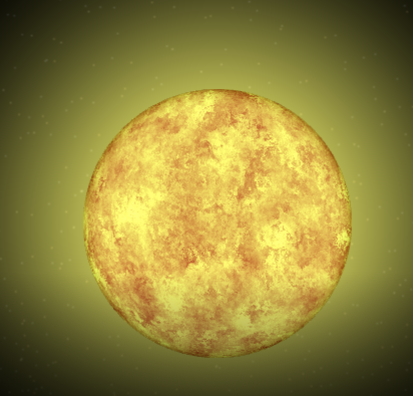
\includegraphics[scale=0.2]{Imagenes/9}
    \caption{Estrella}
    \label{fig:puntosdgs}
    \end{figure}

\column{0.4\textwidth}
    Datos puntuales: 
    \begin{itemize}
        \item Tipo - K 
        \item Masa: 0.5T-0.8T
        \item Temperatura: 3.900 y 5.200 K
        \item Dato curioso: estrellas más buscadas. 
    \end{itemize}
    \end{columns}

\end{frame}

\begin{frame}
\frametitle{Características de la estrella}

\begin{figure}[h!]
    \centering
    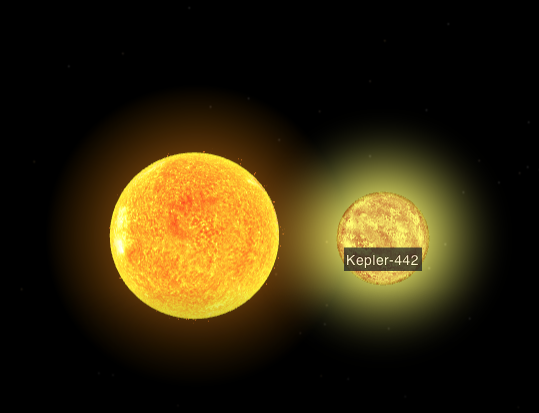
\includegraphics[scale=0.5]{Imagenes/final.png}
    \caption{Comparación al sol}
    \label{fig:jeje}
    \end{figure}
\end{frame}


\section{Referencias}
\begin{frame}[allowframebreaks]{Referecias}
    \begin{thebibliography}{}

        
        \bibitem{uno}
        Torres, Guillermo, et al. 
        \newblock \enquote{Validation of 12 small Kepler transiting planets in the habitable zone.}.
        \newblock  2015. 
        Recuperado de: https://ui.adsabs.harvard.edu/abs/2015ApJ...800...99T/abstract
        
        \bibitem{dos}
        Exoplanet Exploration NASA 
        \newblock \enquote{Kepler 442b}.
        \newblock  2020.
         Recuperado de: https://exoplanets.nasa.gov/exoplanet-catalog/4906/kepler-442-b/
    

    \end{thebibliography}
\end{frame}
\end{document}